\documentclass[10pt,landscape]{article}
\usepackage{multicol}
\usepackage{graphicx}
\usepackage{calc}
\usepackage{ifthen}
\usepackage{color}
\usepackage[landscape]{geometry}

\ifthenelse{\lengthtest { \paperwidth = 11in}}
	{ \geometry{top=.5in,left=.5in,right=.5in,bottom=.5in} }
	{\ifthenelse{ \lengthtest{ \paperwidth = 297mm}}
		{\geometry{top=1cm,left=1cm,right=1cm,bottom=1cm} }
		{\geometry{top=1cm,left=1cm,right=1cm,bottom=1cm} }
	}

% Turn off header and footer
\pagestyle{empty}
 

% Redefine section commands to use less space
\makeatletter
\renewcommand{\section}{\@startsection{section}{1}{0mm}%
                                {-1ex plus -.5ex minus -.2ex}%
                                {0.5ex plus .2ex}%x
                                {\normalfont\large\bfseries}}
\renewcommand{\subsection}{\@startsection{subsection}{2}{0mm}%
                                {-1explus -.5ex minus -.2ex}%
                                {0.5ex plus .2ex}%
                                {\normalfont\normalsize\bfseries}}
\renewcommand{\subsubsection}{\@startsection{subsubsection}{3}{0mm}%
                                {-1ex plus -.5ex minus -.2ex}%
                                {1ex plus .2ex}%
                                {\normalfont\small\bfseries}}
\makeatother

% Define BibTeX command
\def\BibTeX{{\rm B\kern-.05em{\sc i\kern-.025em b}\kern-.08em
    T\kern-.1667em\lower.7ex\hbox{E}\kern-.125emX}}

% Don't print section numbers
\setcounter{secnumdepth}{0}


\setlength{\parindent}{0pt}
\setlength{\parskip}{0pt plus 0.5ex}


% -----------------------------------------------------------------------

\begin{document}

\raggedright
\footnotesize
\begin{multicols}{3}


% multicol parameters
% These lengths are set only within the two main columns
%\setlength{\columnseprule}{0.25pt}
\setlength{\premulticols}{1pt}
\setlength{\postmulticols}{1pt}
\setlength{\multicolsep}{1pt}
\setlength{\columnsep}{2pt}

\begin{center}
   
\includegraphics[width=15px]{emer.png}\huge{\textbf{mergent reference}} \\
   
\end{center}

\section{Keyboard shortcuts}
\subsection{Global project}
\begin{tabular}{@{}ll@{}}
\verb!Ctrl+s!    & Save project. \\
\verb!Ctrl+left! & Backwards in navigation history \\
\verb!Ctrl+right! & Forwards in navigation history \\
\verb!F5!  & Refresh. \\
\verb!Tab! & Forward through interface \\
\verb!Shift+Tab! & Backwards through interface
\end{tabular}

\subsection{Tree browser and program code}
\newlength{\MyLen}
\settowidth{\MyLen}{\texttt{letterpaper}/\texttt{a4paper} \ }
\begin{tabular}{@{}ll@{}}
\verb!Any 1-3 chars!    & Find as you type \\
\verb!Alt+f!  & Find from selected node. \\
\verb!Ctrl+i!    & New item below cursor. \\
\verb!Ctrl+f!  & Expand this node. \\
\verb!Shift++!  & Expand this node. \\
\verb!Ctrl+b!  & Collapse this node. \\
\verb!-!  & Collapse this node. \\
\verb!Ctrl+spacebar!  & Selection mode. \\
\verb!Ctrl+p!  & (select) Previous element. \\
\verb!Ctrl+n!  & (select) Next element. \\
\verb!Ctrl+d!  & Delete selected item(s). \\
\verb!Delete!  & Delete selected item(s). \\
\verb!Ctrl+c!  & Copy selected element(s). \\
\verb!Ctrl+x!  & Cut selected element(s). \\
\verb!Ctrl+v!  & Paste element(s). \\
\verb!Ctrl+u!  & Page up. \\
\verb!Ctrl+v!  & Page down. \\
\verb!Ctrl+g!  & Deselect. \\
\verb!Esc!  & Deselect.
\end{tabular}

\subsection{New elements in left tree browser}
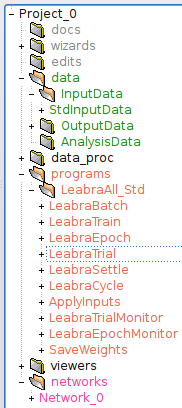
\includegraphics[width=66px]{treebrowser.png} \\
\begin{tabular}{@{}ll@{}}
\verb!do Ctrl+i!    & New Doc \\
\verb!da Ctrl+i!    & New DataTable \\
\verb!la Ctrl+i!    & New Layer \\
\verb!P Ctrl+i!    & New Project \\
\verb!pr Ctrl+i!    & New Program \\
\verb!n Ctrl+i!    & New Network \\
\verb!sp Ctrl+i!    & New Spec
\end{tabular}

\subsection{New elements in program code}
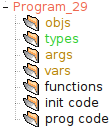
\includegraphics[width=56px]{programcode.png} \\
These sequences insert new items and then take you back. \\
\begin{tabular}{@{}ll@{}}
\verb!obj Ctrl+i Type Ctrl+left,left!    & New obj of Type \\
\verb!var Ctrl+i Ctrl+left,left!    & New var \\
\verb!arg Ctrl+i Ctrl+left,left!    & New arg \\
\verb!fun Ctrl+i Ctrl+left,left!    & New fun \\
\verb!init Ctrl+i Name Ctrl+left,left!    & New init code Name \\
\verb!prog Ctrl+i Name Ctrl+left,left!    & New prog code Name \\
\end{tabular}

\subsection{Middle panel edit dialogs}
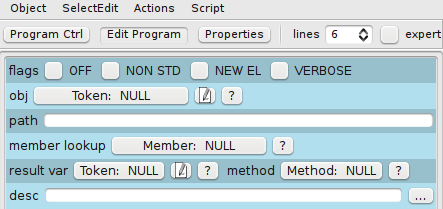
\includegraphics[width=225px]{middlepanel.png} \\
\settowidth{\MyLen}{\texttt{multicol} }
\begin{tabular}{@{}ll@{}} \\
\verb!Tab!    & Next element. \\
\verb!Shift+tab!    & previous element. \\
\verb!Up!    & (numeric field) Increase value. \\
\verb!Down!    & (numeric field) Decrease value. \\
\verb!Up!    & (dropdown) Move up. \\
\verb!Down!    & (dropdown) Move down. \\
\verb!ESC!    & Revert changes. \\
\verb!Ctrl+Enter!    & Apply changes. \\
\verb!Spacebar!    & (buttons) Open token chooser. \\
\verb!Spacebar!    & (flags) Check/uncheck flag. \\
\verb!Ctrl+l!    & (expression fields) Lookup information. \\
\end{tabular}

\subsection{3D network and graph viewer}
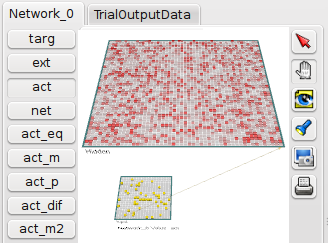
\includegraphics[width=164px]{netview.png} \\
\settowidth{\MyLen}{\texttt{multicol} }
\begin{tabular}{@{}ll@{}}
\verb!i!    & Interact (mouse cursor). \\
\verb!v!    & Camera view (hand). \\
\verb!a!    & View all (eyeball) (broken).\\ 
\verb!s!    & Seek (flashlight) (broken). \\
\verb!Shift+mouse!    & Drag in x,y plane. \\
\verb!Middle mouse scroll!    & Zoom in/out in z plane.
\verb!! \\
\verb!! \\
\end{tabular}

\section{Programing}
\subsection{taDataProc::}
\subsubsection{Columns category}
\verb!ConcatCols ( DataTable* dest, DataTable* src_a,...)!\\ \ \ Concat two tables, preserving all data
\verb!Join(DataTable* dest,DataTable* src_a,DataTable* src_b,...)!\\\ \ \ Left, right and inner join two tables
\subsubsection{Copy category}
\verb!AppendRows(DataTable* dest,DataTable* src)!\\\ \ \ Append rows of src to dest
\verb!ConcatRows(DataTable* dest,DataTable* src_a, ...)!\\\ \ \ Concatenate rows from all src tables into dest
\verb!CopyCommonColData(DataTable* dest,DataTable* src)!\\\ \ \ Append data from src to dest for all common cols
\verb!CopyCommonColsRow(DataTable* dest,DataTable* src,!\\\ \ \ \ \ \ \ \ \ \ \ \ \ \ \ \ \ \ \ \ \ \ \ \ \ \ \ \verb!int dest_row, int src_row)!\\\ \ \ Append data from src to dest for all common cols
\verb!CopyData(DataTable* dest,DataTable* src)!\\\ \ \ Destructively copy data from src to dest
\verb!ReplicateRows(DataTable* dest,DataTable* src,int n_repl)!\\\ \ \ Destructively replicate rows of src into dest n\_repl times
\subsubsection{Order category}
\verb!Group(DataTable* dest,DataTable* src,DataGroupSpec* spec)!\\\ \ \ Group data from src into dest according to spec
\verb!Permute(DataTable* dest, DataTable* src)!\\\ \ \ Randomly reorder the rows of src table into dest
\verb!Sort(DataTable* dest,DataTable* src,DataSortSpec* spec)!\\\ \ \ Sort src data into dest according to sort spec 
\verb!SortInPlace(DataTable* dt,DataSortSpec* spec)!\\\ \ \  Sort data in place according to sort spec
\subsubsection{Select category}
\verb!SelectRows(DataTable* dest,DataTable* src,DataSelectSpec* spec)!\\\ \ \ Select rows of src into dest according to spec
\verb!SplitRows(DataTable* dest_a,DataTable* dest_b,...)!\\\ \ \ Split src rows that mach spec into dest\_b, otherwise dest\_a

\subsection{taDataGen::}
\subsubsection{Basic category}
\verb!Clear(DataTable* data,const taString& col_nm,float val=0.0)!\\\ \ \ Clear all data. Set all data to val if provided.
\verb!SimpleMath(DataTable* data,const taString& col_nm,...)!\\\ \ \ Apply simple math op to all vals in float\_Matrix col
\subsubsection{Distance category}
\verb!LastMinDist(DataCol* da,int row,...)!\\\ \ \ returns min distance between nth pattern and all previous
\verb!LastMinMaxDist(DataCol* da,int row,float& max_dist,...)!\\\ \ \ Returns min and max distance between nth patte
\subsubsection{Draw category}
\verb!RenderLine(float_Matrix* mat,int xs, int ys, int xe,...)!\\\ \ \ Render a line from,to start,end
\verb!RenderWideLine(float_Matrix* mat,int xs, int ys,...)!\\\ \ \ Render a wide line from,to start,end
\verb!WritePoint(float_Matrix* mat,int x,int y,...)!\\\ \ \ Write a single point
\subsubsection{Files category}
\verb!GetDirFiles(DataTable* dest,...)!\\\ \ \ Read file names from given directory into rows of the data table
\subsubsection{Lists category}
\verb!CombineFrequencies(DataTable* freq_output,...)!\\\ \ \ Operate on input items,freqs into output freqs
\verb!CrossLists(DataTable* crossed_output,...)!\\\ \ \ Creates a full set of combination of elements from two or more lists. \\
\verb!ProbSelectColNo(DataTable* data_table,...)!\\\ \ \ Select a column number from data table based on probabilities associated with different columns.
\verb!ProbSelectRow(DataTable* data_table,...)!\\\ \ \ Randomly generate events based on a set of probabilitis for given options at each point.
\verb!ReplicateByFrequency(DataTable* repl_output,...)!\\\ \ \ Replicate input by the number in the frequency column times the total\_number value.
\verb!SampleByFrequency(DataTable* repl_output,...)!\\\ \ \ Sample the items in the input data as a function of the probability value given in the frequency column, with n\_samples taken per row .
\verb!SortedPermutations(DataTable* dest, int n)!\\\ \ \ Generate a sorted list of all possible n! permutations of the digits 1..n in sorted order and write them to destination data table dest.
\subsubsection{Random category}
\verb!AddNoise(DataTable* data,...)!\\\ \ \ Add random noise of specified type to the patterns.
\verb!AddNoiseMat(float_Matrix* mat,...)!\\\ \ \ Add random noise to given pattern.
\verb!FlipBits(DataTable* data,...)!\\\ \ \ Flip n\_off bits from 1's to 0's, and n\_on bits from 0's to 1's in float matrix column col\_nm.
\verb!FlipBitsMat(float_Matrix* mat,...)!\\\ \ \ Flip n\_off of the 1 bits into the 0 state, and n\_on of the 0 bits to the 1 state.
\verb!PermutedBinary(DataTable* data,...)!\\\ \ \ Create permuted binary patterns of n\_on on\_vals (1's) and rest off\_vals (0's) in given col (must be float matrix).
\verb!PermutedBinaryMat(float_Matrix* mat,...)!\\\ \ \ Set matrix values to permuted binary pattern of n\_on on\_vals and rest off\_vals.
\verb!PermutedBinary_MinDist(DataTable* data,...)!\\\ \ \ Create permuted binary patterns with dist minimum hamming distance (or dist max\_correl).
\subsubsection{SubMatrix category}
\verb!ReadToSubMatricies(DataTable* src,...)!\\\ \ \ For making larger patterns out of smaller ones (sub-matricies) and vice-versa.
\verb!WriteFmSubMatricies(DataTable* dest,...)!\\\ \ \ For making larger patterns out of smaller ones (sub-matricies) and vice-versa.

\subsection{taDataAnal::}
\subsubsection{Clean category}
\verb!SmoothExp(DataTable* smooth_data,...)!\\\ \ \ Exponential smoothing: compute the exponentially-convolved average for all the numeric fields of source data, using an exponential kernel of given half-width and exponent.\\
\verb!SmoothGauss(DataTable* smooth_data,...)!\\\ \ \ Gaussian smoothing
\verb!SmoothPow(DataTable* smooth_data,...)!\\\ \ \ Power-function smoothing
\verb!SmoothUniform(DataTable* smooth_data!,...)\\\ \ \ Uniform smoothing
\verb!TimeAvg(DataTable* time_avg_data,...)!\\\ \ \ Compute the time average for all the numeric fields of source data, according to the given avg\_dt.
\subsubsection{Correlation category}
\verb!CorrelMatrix(float_Matrix* correl_mat,...)!\\\ \ \ Compute correlation matrix across rows for given matrix data column in src\_data datatable.
\subsubsection{Distance category}
\verb!CrossDistMatrix(float_Matrix* dist_mat,...)!\\\ \ \ Compute cross distance matrix between two different matrix data columns in src\_data\_a and src\_data\_b datatables.
\verb!DistMatrix(float_Matrix* dist_mat,...)!\\\ \ \ Compute distance matrix for given matrix data column in src\_data datatable.
\subsubsection{Graph}
\verb!Matrix3DGraph(DataTable* data,...)!\\\ \ \ Prepare data for a 3D matrix graph, where data is plotted by X and Z axis values -- sorts data by X then Z, then adds a duplicate copy of data sorted by Z then X, which produces a matrix grid in a graph view plot (turn off the Z neg draw flag).
\subsubsection{HighDim}
\verb!Cluster(DataTable* clust_data,...)!\\\ \ \ Produce a hierarchical clustering of the distances between patterns in given data column from source data, with labels from given name\_col\_nm, using given distance metric.
\verb!MDS2dPrjn(DataTable* prjn_data,...)!\\\ \ \ Perform multidimensional scaling on the distance matrix (computed according to metric, norm, tol parameters) of patterns in column name across rows, putting the resulting projections into prjn\_data.
\verb!PCA2dPrjn(DataTable* prjn_data,...)!\\\ \ \ Perform principal components analysis of the correlations of patterns in given columm across rows, plotting projections of patterns on the given principal components in the data table.
\verb!PCAEigens(float_Matrix* eigen_vals,...)!\\\ \ \ Get principal components analysis (PCA) eigenvalues and eigenvectors of correlation matrix across rows for given matrix column name in source data
\verb!RowPat2dPrjn(DataTable* prjn_data,...)!\\\ \ \ Project all rows according to their projection onto the two specified rows of patterns using given distance metrics.
\subsubsection{Stats}
\verb!RegressLinear(DataTable* src_data,...)!\\\ \ \ Compute linear regression (least squares fit of function y = mx + b) to given data.

\subsection{Program code elements}
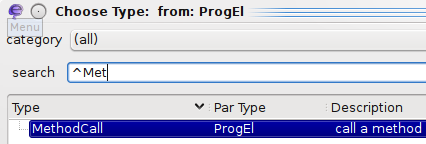
\includegraphics[width=137px]{progel.png} \\
Press Ctrl+i seq Enter as fast as you can, where seq is defined below as the shortest sequence needed to put that program element at the top of the chooser list. No need to wait for visual confirmation of the choice.
\subsubsection{Ctrl}
\begin{tabular}{@{}ll@{}}
\verb!ForLoop!    & f. \\
\verb!DoLoop!    & do. \\
\verb!WhileLoop!    & w. \\
\verb!If!    & ife. \\
\verb!IfCont!    & ifc. \\
\verb!IfBreak!    & ifb. \\
\verb!IfReturn!    & ifr. \\
\verb!CodeBlock!    & co. \\
\verb!UserScript!    & u. \\
\end{tabular}
\subsubsection{Var/Fun}
\begin{tabular}{@{}ll@{}}
\verb!ProgVars!    & progvars. \\
\verb!AssignExpr!    & as. \\
\verb!VarIncr!    & v. \\
\verb!MemberAssign!    & me. \\
\verb!MethodCall!    & met. \\
\verb!MemberMethodCall!    & me Tab Ctrl+n,n. \\
\verb!FunctionCall!    & fu Tab Ctrl+n. \\
\verb!ReturnExpr!    & ret. \\
\verb!ProgramCall!    & prog Tab Ctrl+n,n. \\
\verb!ProgramCallVar!    & prog Tab Ctrl+n,n,n. \\
\verb!OtherProgramVar!    & prog Tab Ctrl+n,n,n.
\end{tabular}
\subsubsection{Print/Args}
\begin{tabular}{@{}ll@{}}
\verb!PrintExpr!    & p. \\
\verb!PrintVar!    & p Tab Ctrl+n. \\
\verb!Comment!    & com. \\
\verb!StopStepPoint!    & sto. \\
\verb!ProgVarFmArg!    & pro. \\
\verb!MemberFmArg!    & me Tab Ctrl+n. \\
\verb!DataColsFmArgs!    & dataco. \\
\verb!RegisterArgs!    & re. \\
\end{tabular}
\subsubsection{Misc Fun}
\begin{tabular}{@{}ll@{}}
\verb!StaticMethodCall!    & st. \\
\verb!MathCall!    & m. \\
\verb!RandomCall!    & r. \\
\verb!MiscCall!    & mi. \\
\verb!DataProcCall!    & datap. \\
\verb!DataAnalCall!    & d. \\
\verb!DataGenCall!    & datag. \\
\verb!ImageProcCall!    & im. \\
\end{tabular}
\subsubsection{Data}
\begin{tabular}{@{}ll@{}}
\verb!DataLoop!    & datal. \\
\verb!ResetDataRows!    & res. \\
\verb!AddNewDataRow!    & a. \\
\verb!DoneWritingDataRow!    & don. \\
\verb!DataVarProg!    & datav. \\
\verb!DataVarProgMatrix!    & datav Tab Ctrl+n. \\
\end{tabular}

\verb!! \\
\verb!! \\
\verb!! \\
\verb!! \\
\verb!! \\
\verb!! \\
\verb!! \\
\verb!! \\
\verb!! \\
\verb!! \\
\verb!! \\
\verb!! \\
\verb!! \\
\verb!! \\
\verb!! \\
\verb!! \\
\verb!! \\
\verb!! \\
\verb!! \\
\verb!! \\
\verb!! \\
\verb!! \\
\verb!! \\
\verb!! \\
\verb!! \\
\verb!! \\
\verb!! \\
\verb!! \\
\verb!! \\
\verb!! \\
\verb!! \\
\verb!! \\
\verb!! \\
\verb!! \\
\verb!! \\
\verb!! \\
\verb!! \\
\verb!! \\
\verb!! \\
\verb!! \\
\verb!! \\
\verb!! \\
\verb!! \\
\verb!! \\
\verb!! \\
\verb!! \\
\verb!! \\
\verb!! \\
\verb!! \\
\verb!! \\
\verb!! \\
\verb!! \\
\verb!! \\
\verb!! \\
\verb!! \\
\verb!! \\
\verb!! \\
\verb!! \\
\verb!! \\
\verb!! \\
\verb!! \\
\verb!! \\
\verb!! \\
\verb!! \\
\verb!! \\
\verb!! \\
\verb!! \\
\verb!! \\
\verb!! \\
\verb!! \\
\verb!! \\
\verb!! \\
\verb!! \\
\verb!! \\
\verb!! \\
\verb!! \\
\verb!! \\
\verb!! \\
\verb!! \\
\verb!! \\
\verb!! \\
\verb!! \\
\verb!! \\
\verb!! \\
\verb!! \\
\verb!! \\
\verb!! \\
\verb!! \\
\verb!! \\
\verb!! \\
\verb!! \\
\verb!! \\
\verb!! \\
\verb!! \\
\verb!! \\
\verb!! \\
\verb!! \\
\verb!! \\
\verb!! \\
\verb!! \\
\verb!! \\
\verb!! \\
\verb!! \\
\verb!! \\
\verb!! \\
\verb!! \\
\verb!! \\
\verb!! \\
\verb!! \\
\verb!! \\
\verb!! \\
\verb!! \\
\verb!! \\
\verb!! \\
\verb!! \\
\verb!! \\
\verb!! \\
\verb!! \\
\verb!! \\
\verb!! \\
\verb!! \\
\verb!! \\
\verb!! \\
\verb!! \\
\verb!! \\
\verb!! \\
\verb!! \\
\verb!! \\
\verb!! \\
\verb!! \\
\verb!! \\
\verb!! \\
\verb!! \\
\verb!! \\
\verb!! \\
\verb!! \\
\verb!! \\
\verb!! \\
\verb!! \\
\verb!! \\
\verb!! \\
\verb!! \\
\verb!! \\
\end{multicols}
\end{document}
